\section{Resultados}

\subsection{Sobre la climatología del tamaño de los CTs}
\begin{frame}
\begin{itemize}
    \item Se analizaron {\red 191} y {\gray 337} CTs de las cuencas {\red NA} y {\gray EP} respectivamente durante el periodo 2000-2020.
    \\~\
    \item Sólo se consideran las posiciones de CT de 6 horas que se localizan en la región de estudio. Se obtuvieron {\red 4526} y {\gray 6923} posiciones de CTs para las cuencas.
\end{itemize}
\end{frame}

\begin{frame}
    \begin{figure}
        \centering
        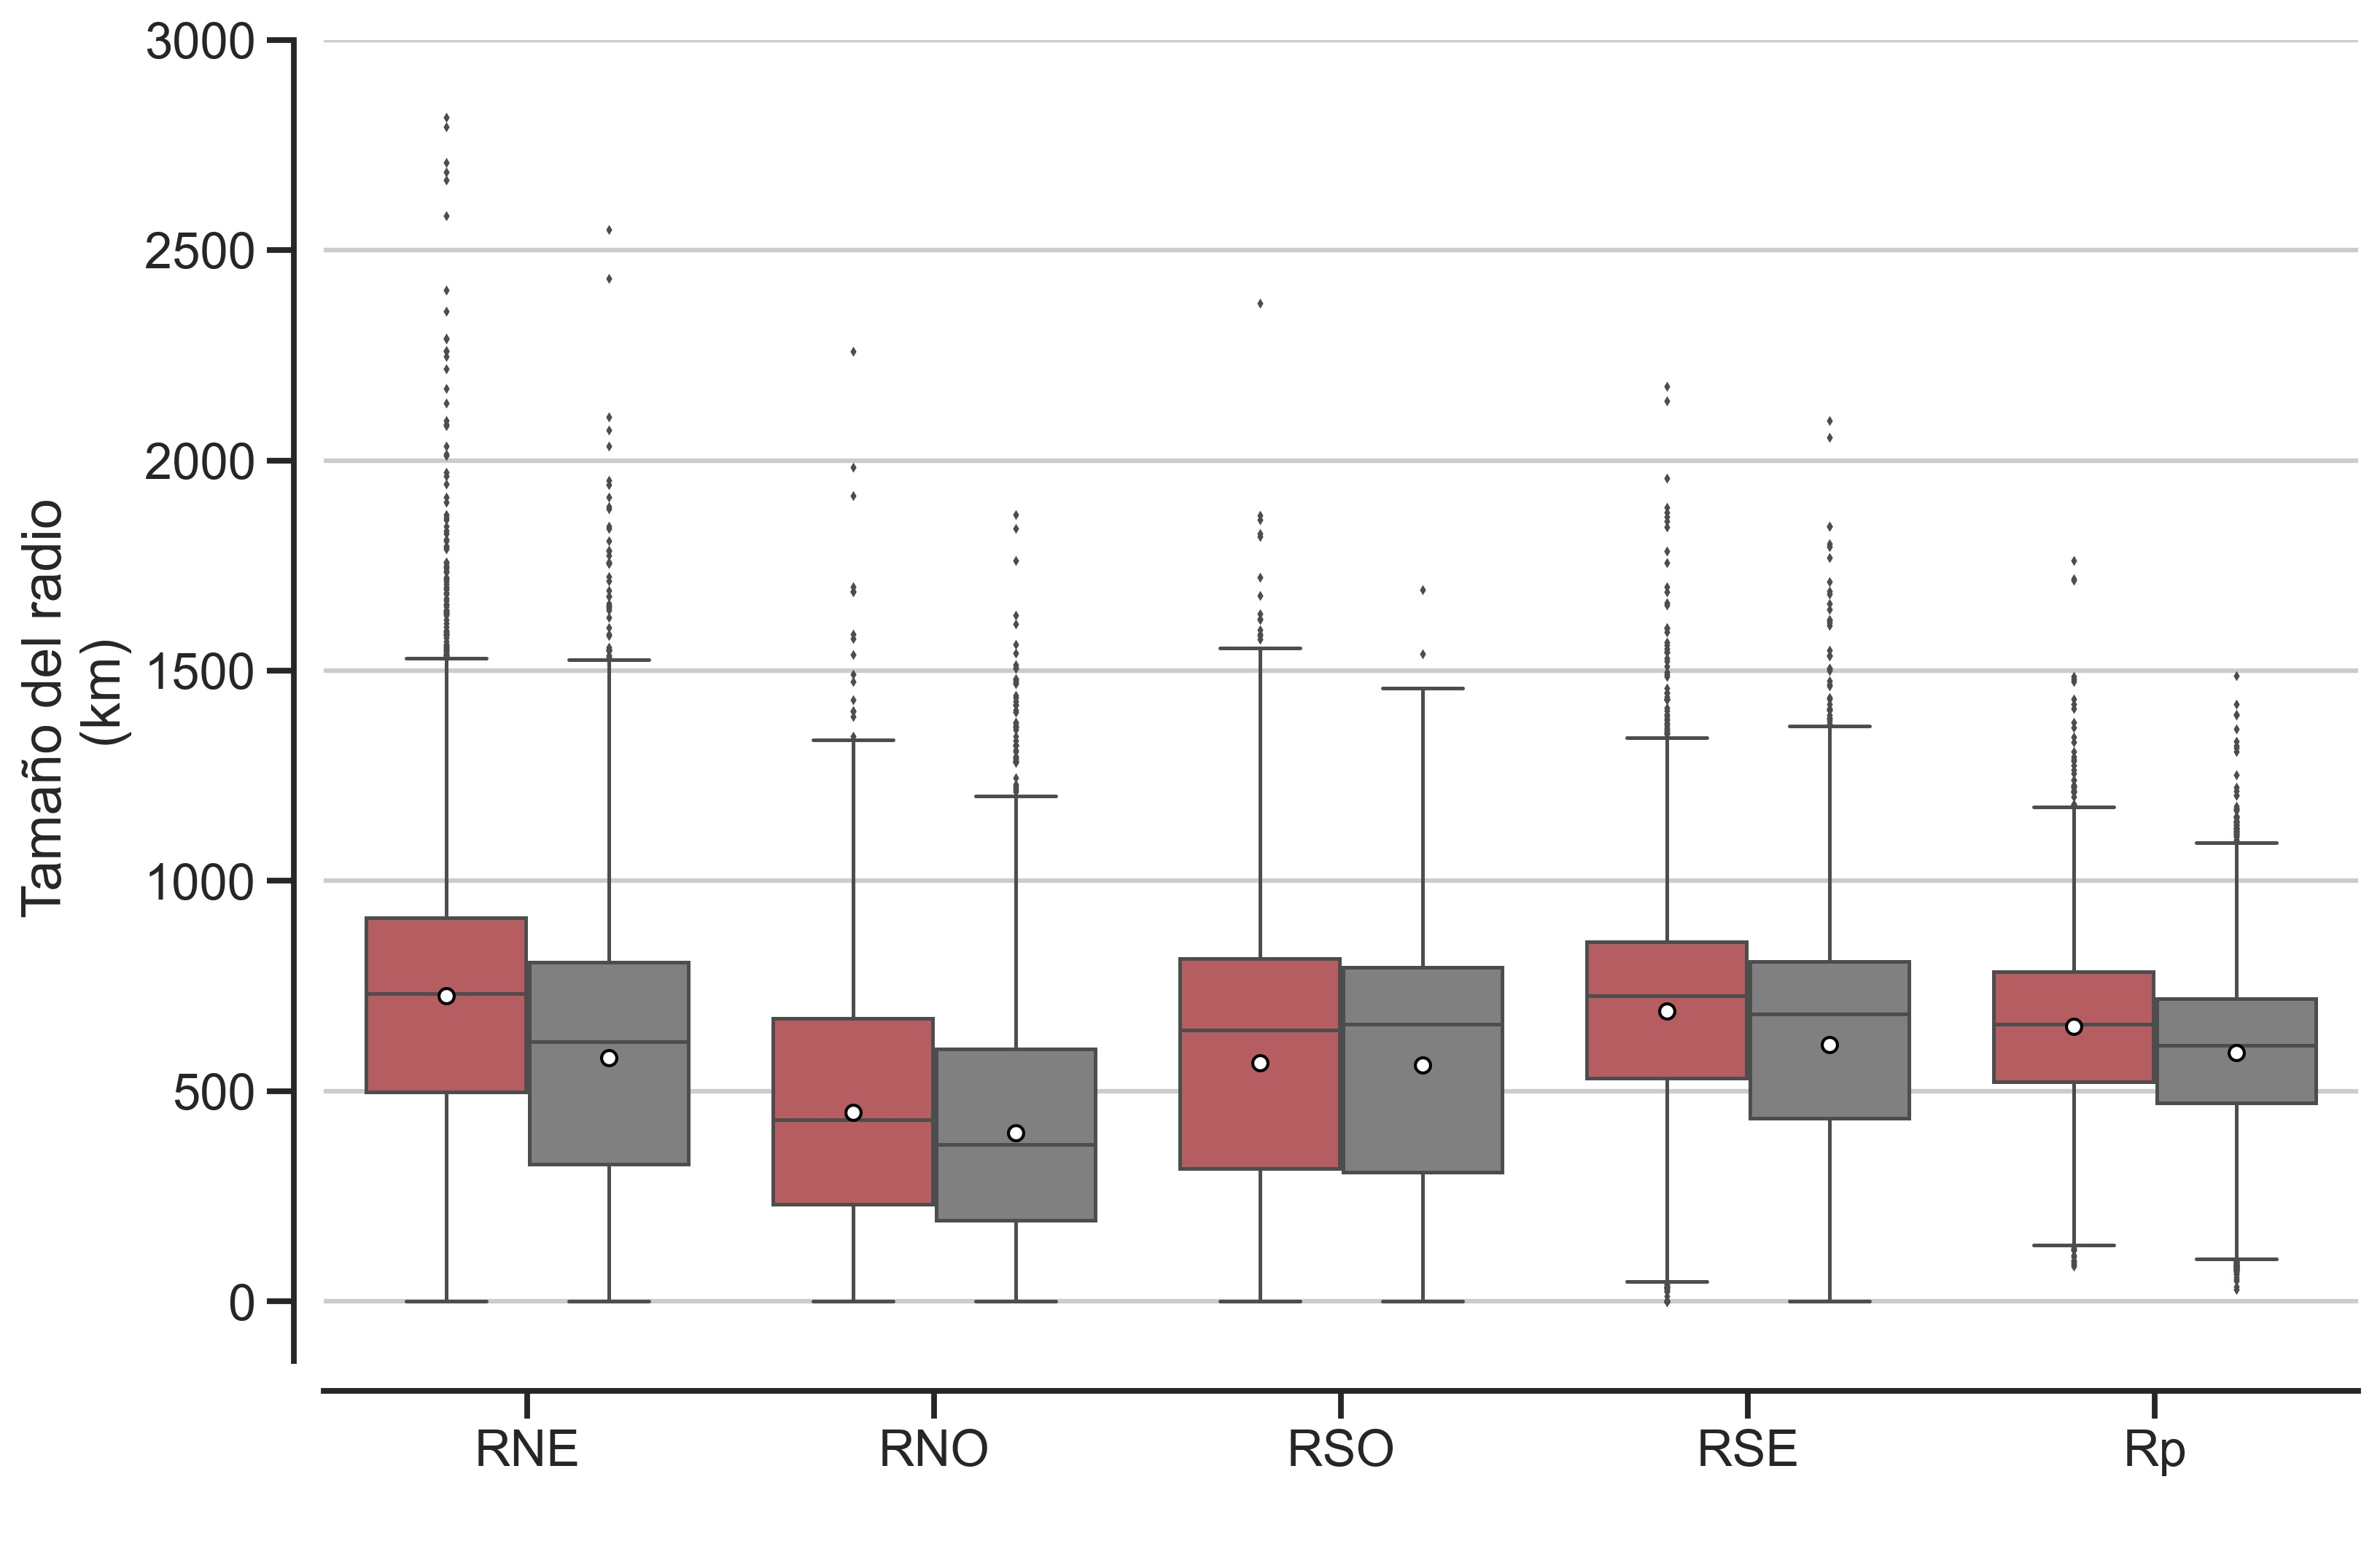
\includegraphics[scale = 0.35]{Images/Figures/Fig_3_1.jpeg}
        \caption{Cajas y bigotes de las distribuciones de los radios por cuadrante y el $R_p$ (km) de los radios en la región de estudio de la cuenca {\red NA} y {\gray EP}.}
        \label{fig:fig_9}
    \end{figure}
\end{frame}

\begin{frame}
    \begin{columns}
        \begin{column}{0.4\textwidth}
            \begin{enumerate}
                \setcounter{enumi}{0}
                \item Sobre la variación espacial de los tamaños
            \begin{block}{Figura 9:}
                Distribución espacial del tamaño de los CTs por cuadrante (km): (a) RNE, (b) RNO, (c) RSO, (d) RSE y (e) $R_p$. Los límites en la barra de colores representan los rangos intercuantilícos (p25 y p75) durante el periodo 2000-2020.
            \end{block}
            \end{enumerate}
        \end{column}
        \begin{column}{0.6\textwidth}
        \begin{figure}
            \centering
            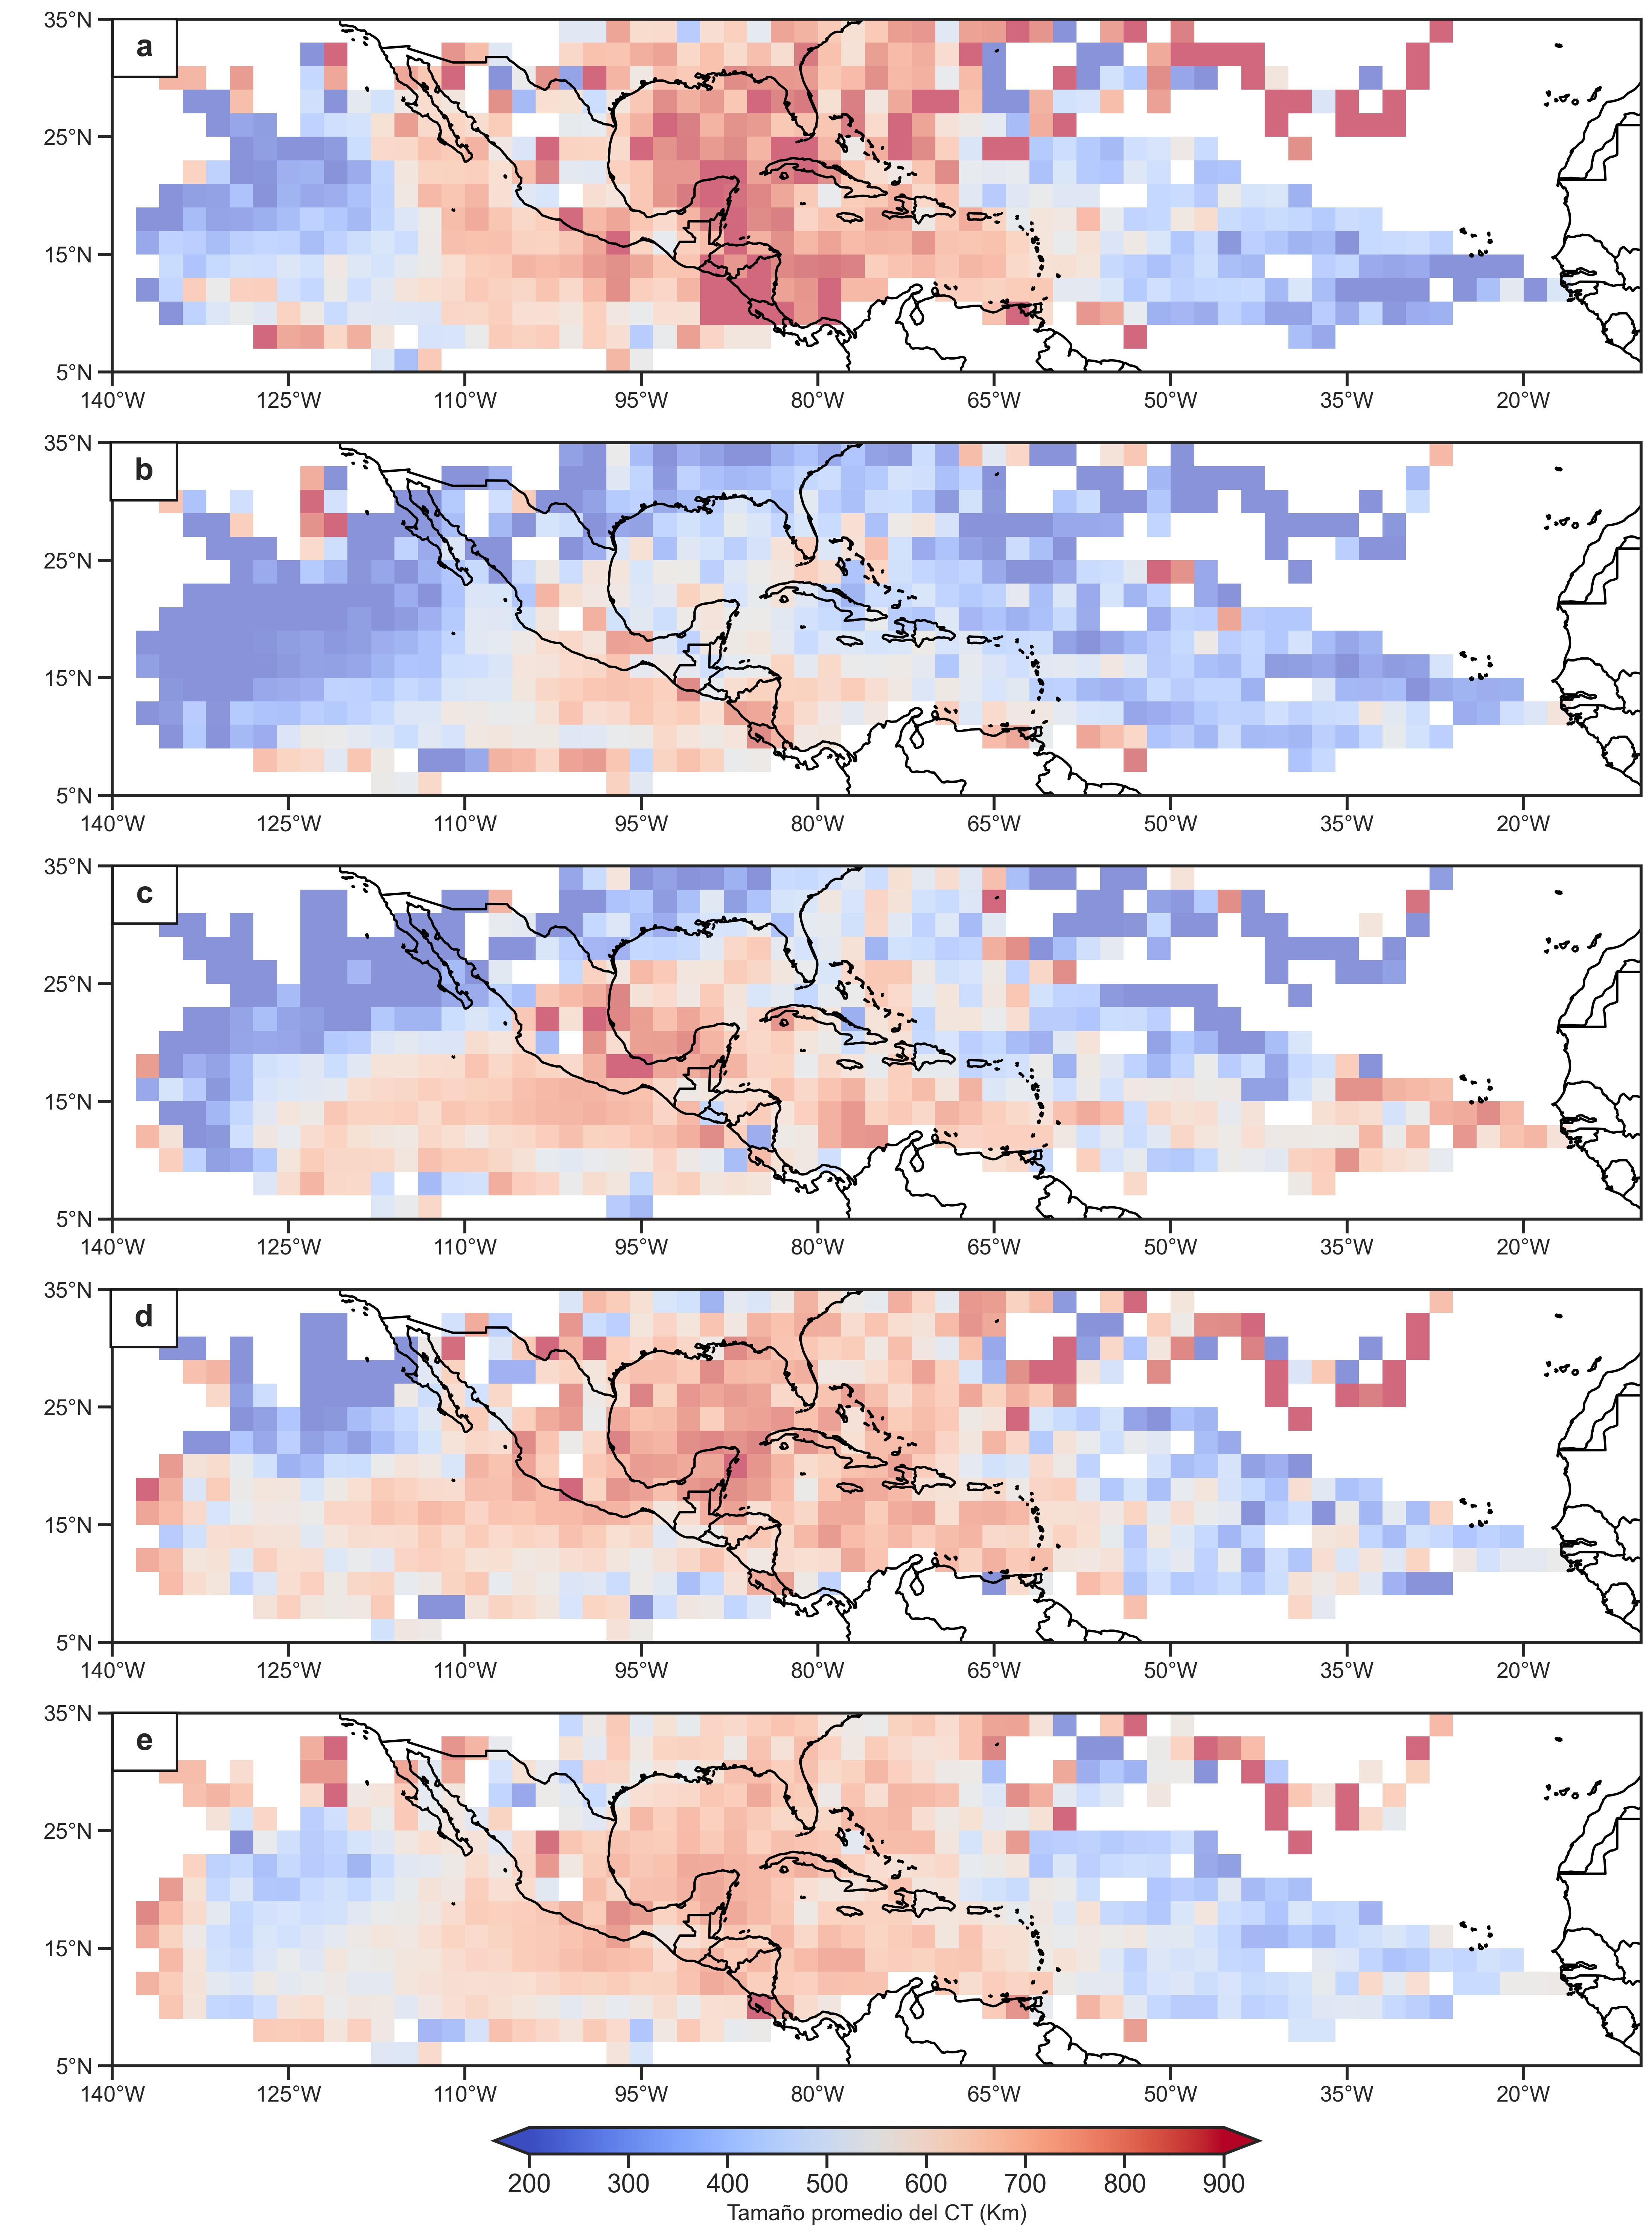
\includegraphics[scale = 0.17]{Images/Figures/Fig_3_6.jpeg}
            \caption{}
            \label{fig:fig_tamaño}
        \end{figure}
        \end{column}
    \end{columns}
\end{frame}

\begin{frame}
    \begin{enumerate}
    \setcounter{enumi}{0}
    \item Sobre la variación espacial de los tamaños
    \begin{figure}
        \centering
        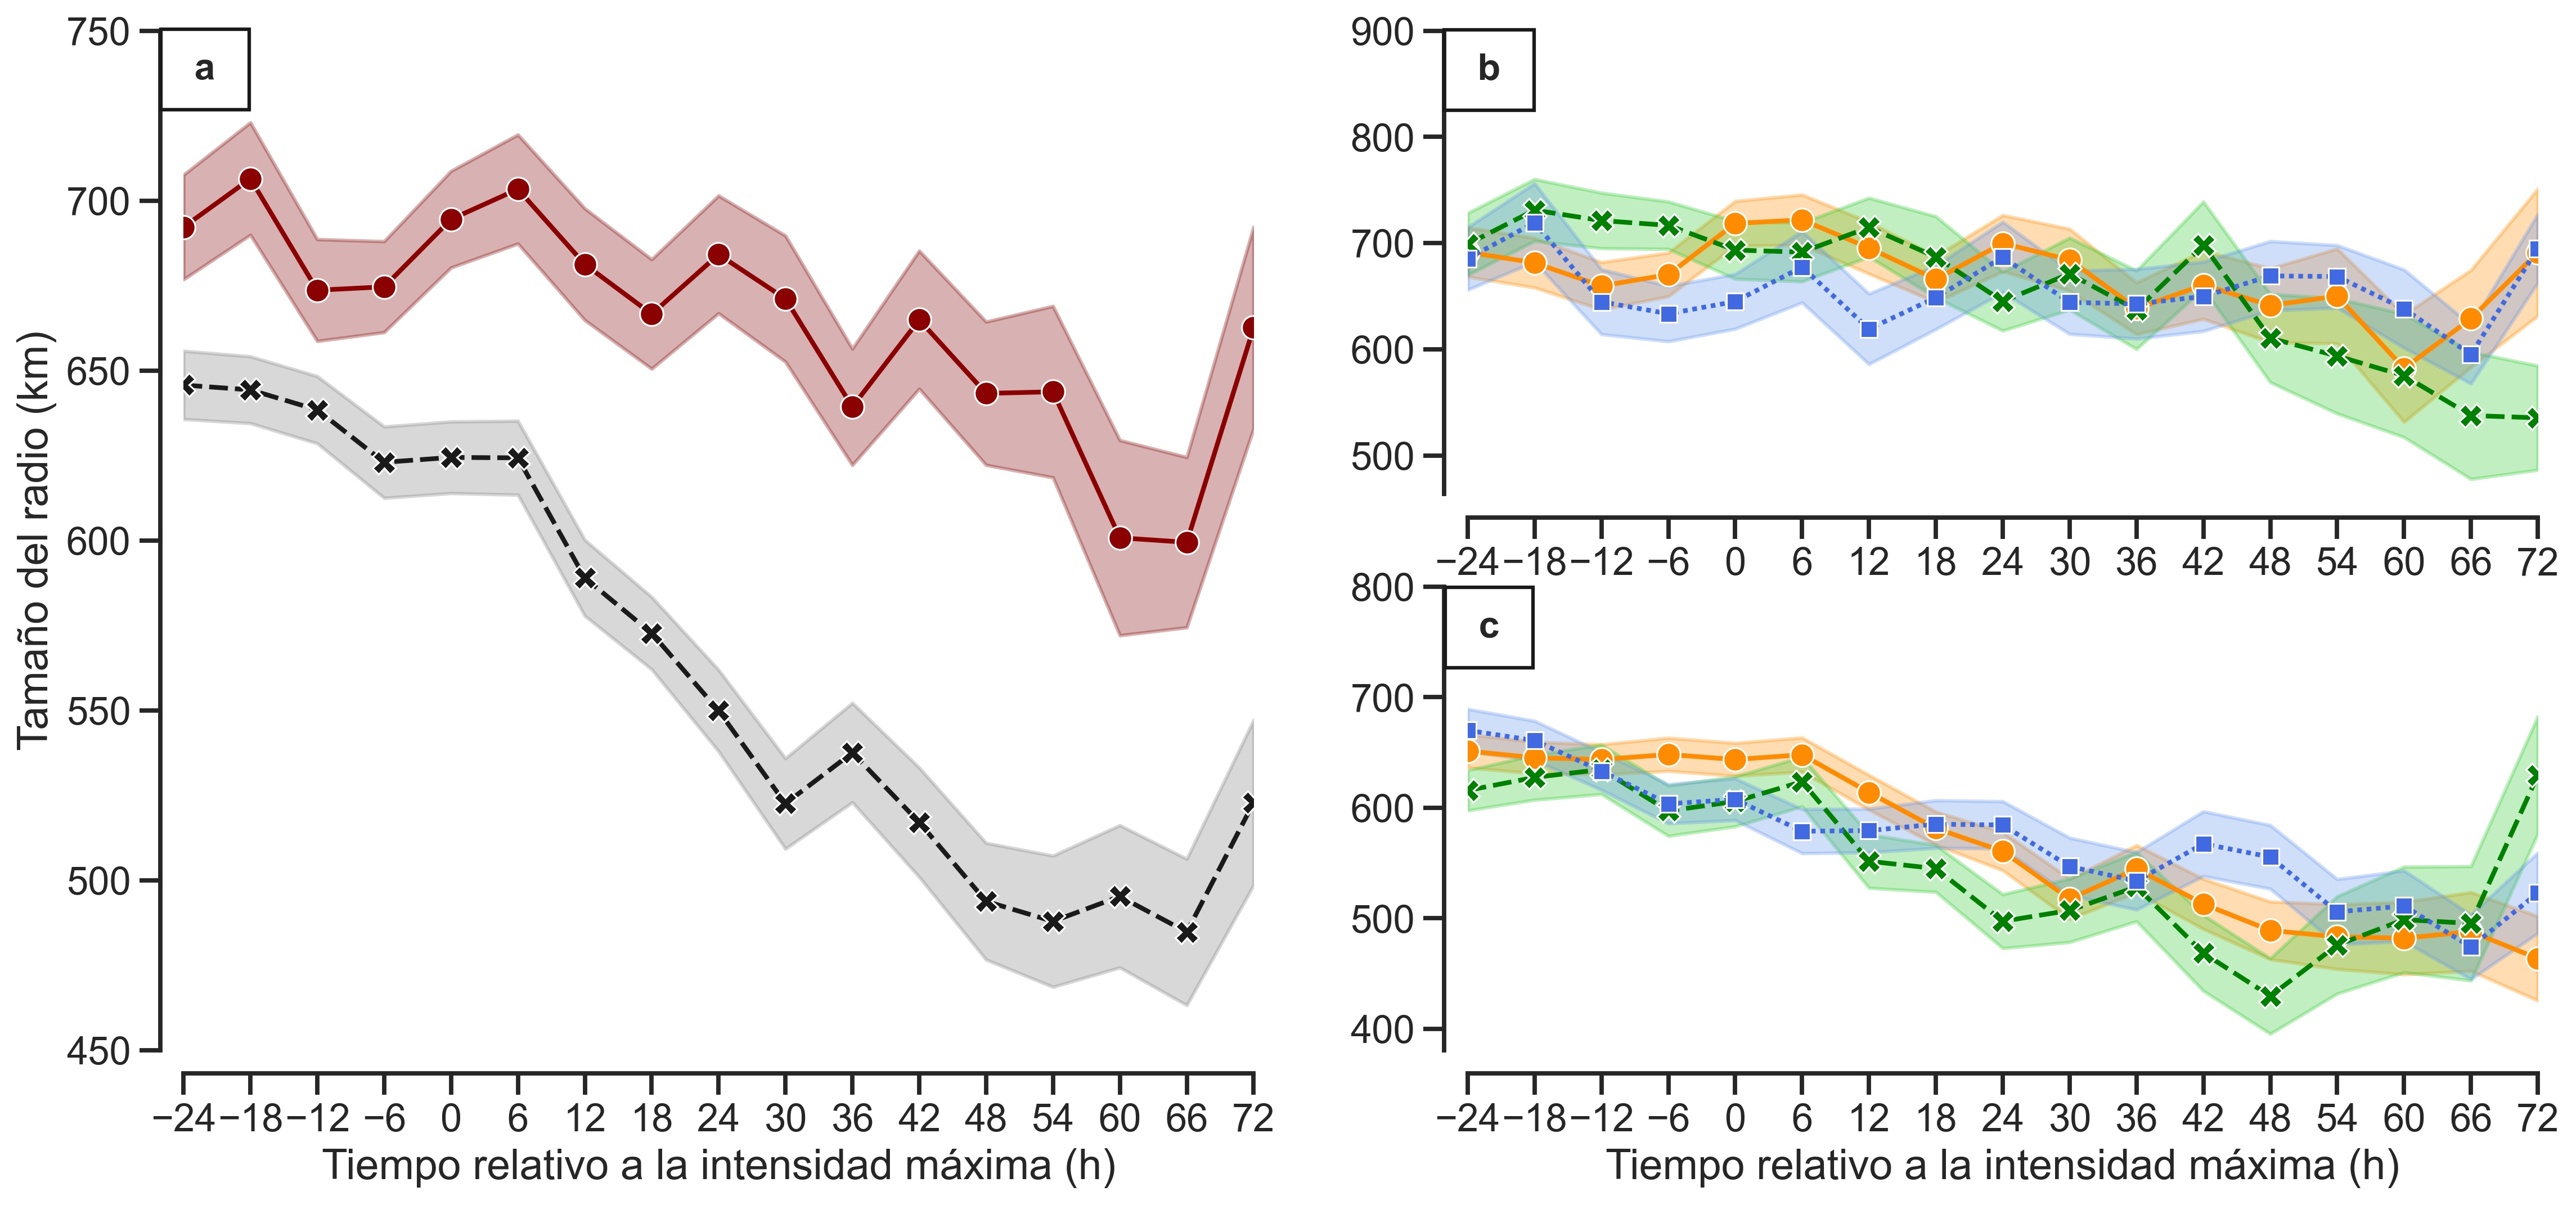
\includegraphics[scale = 0.26]{Images/Figures/Fig_3_8.jpeg}
        \caption{Compuestos de tamaño de Rp (km) de: (a) los CTs sobre {\red NA} y {\gray EP} y las TTs (en amarillo), HUR1-2 (en verde) y HUR3-5 (en azul) sobre (b) {\red NA} y (c) {\gray EP}. El tiempo 0 h representa el momento en que alcanzan la máxima intensidad. Las áreas sombreadas proporcionan el error estándar asociado al valor promedio de $R_p$ cada 6 h.}
        \label{fig:fig_11}
    \end{figure}
    \end{enumerate}
\end{frame}

\begin{frame}
    \begin{enumerate}
    \setcounter{enumi}{1}
        \item Sobre la variación mensual de los tamaños
    \end{enumerate}
    \begin{figure}
        \centering
        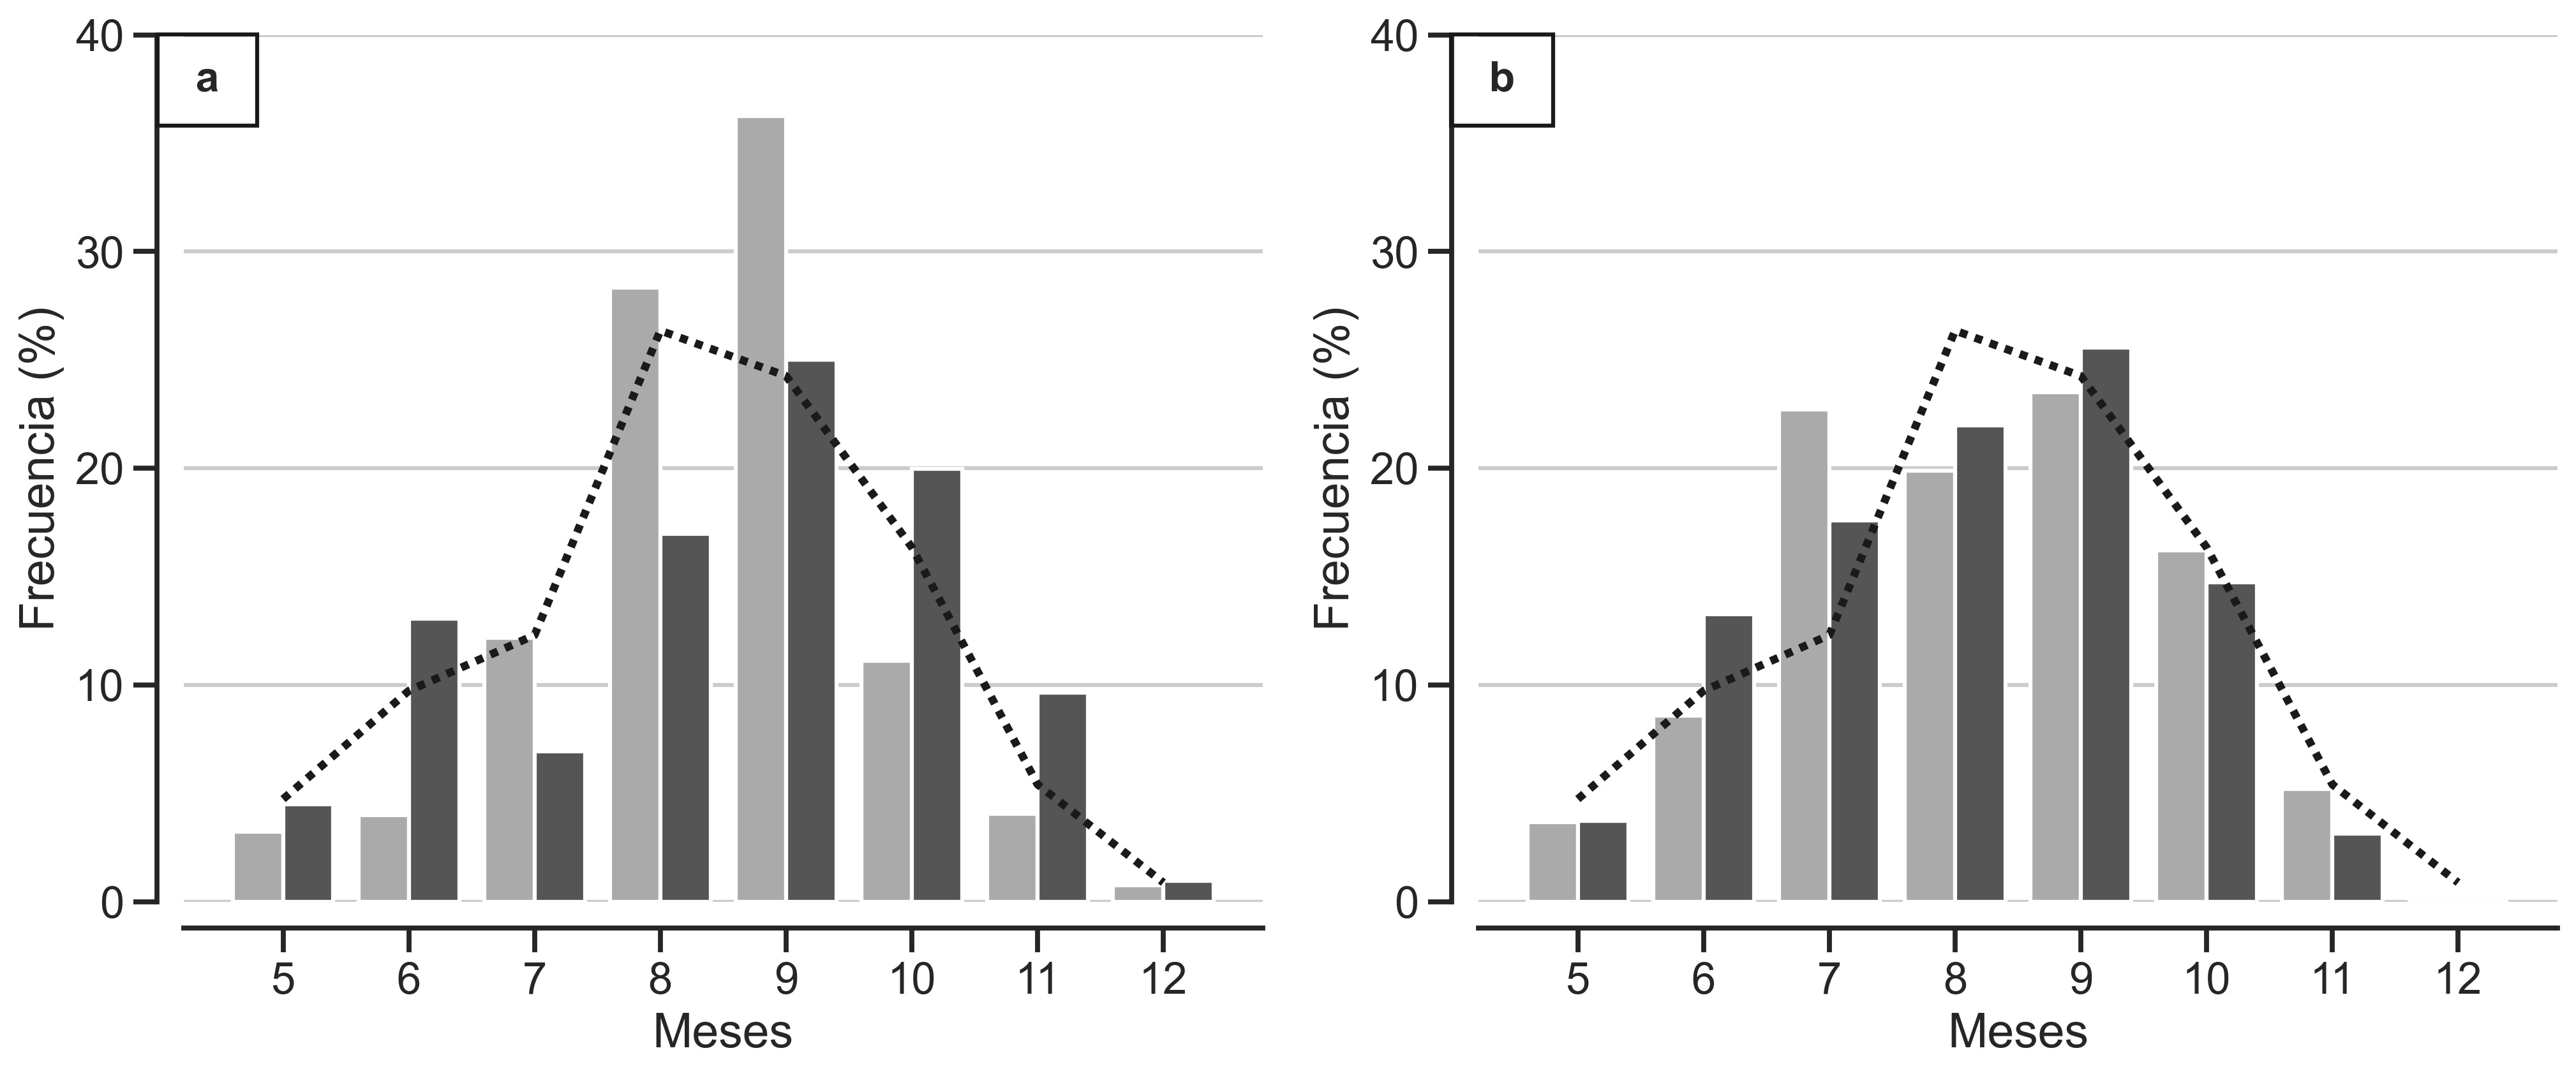
\includegraphics[scale = 0.3]{Images/Figures/Fig_3_10.jpeg}
        \caption{Tamaños mensuales de CT para los cuartiles inferior (pequeño) y superior (grande) en: (a) cuencas {\red NA} y (b) {\gray EP}.}
        \label{fig:fig_12}
    \end{figure}
\end{frame}

\subsection{Sobre la relación del tamaño y la precipitación}
\begin{frame}
\begin{enumerate}
\setcounter{enumi}{0}
    \item Climatología de los tamaños usando productos IMERG
\end{enumerate}
    \begin{figure}
        \centering
        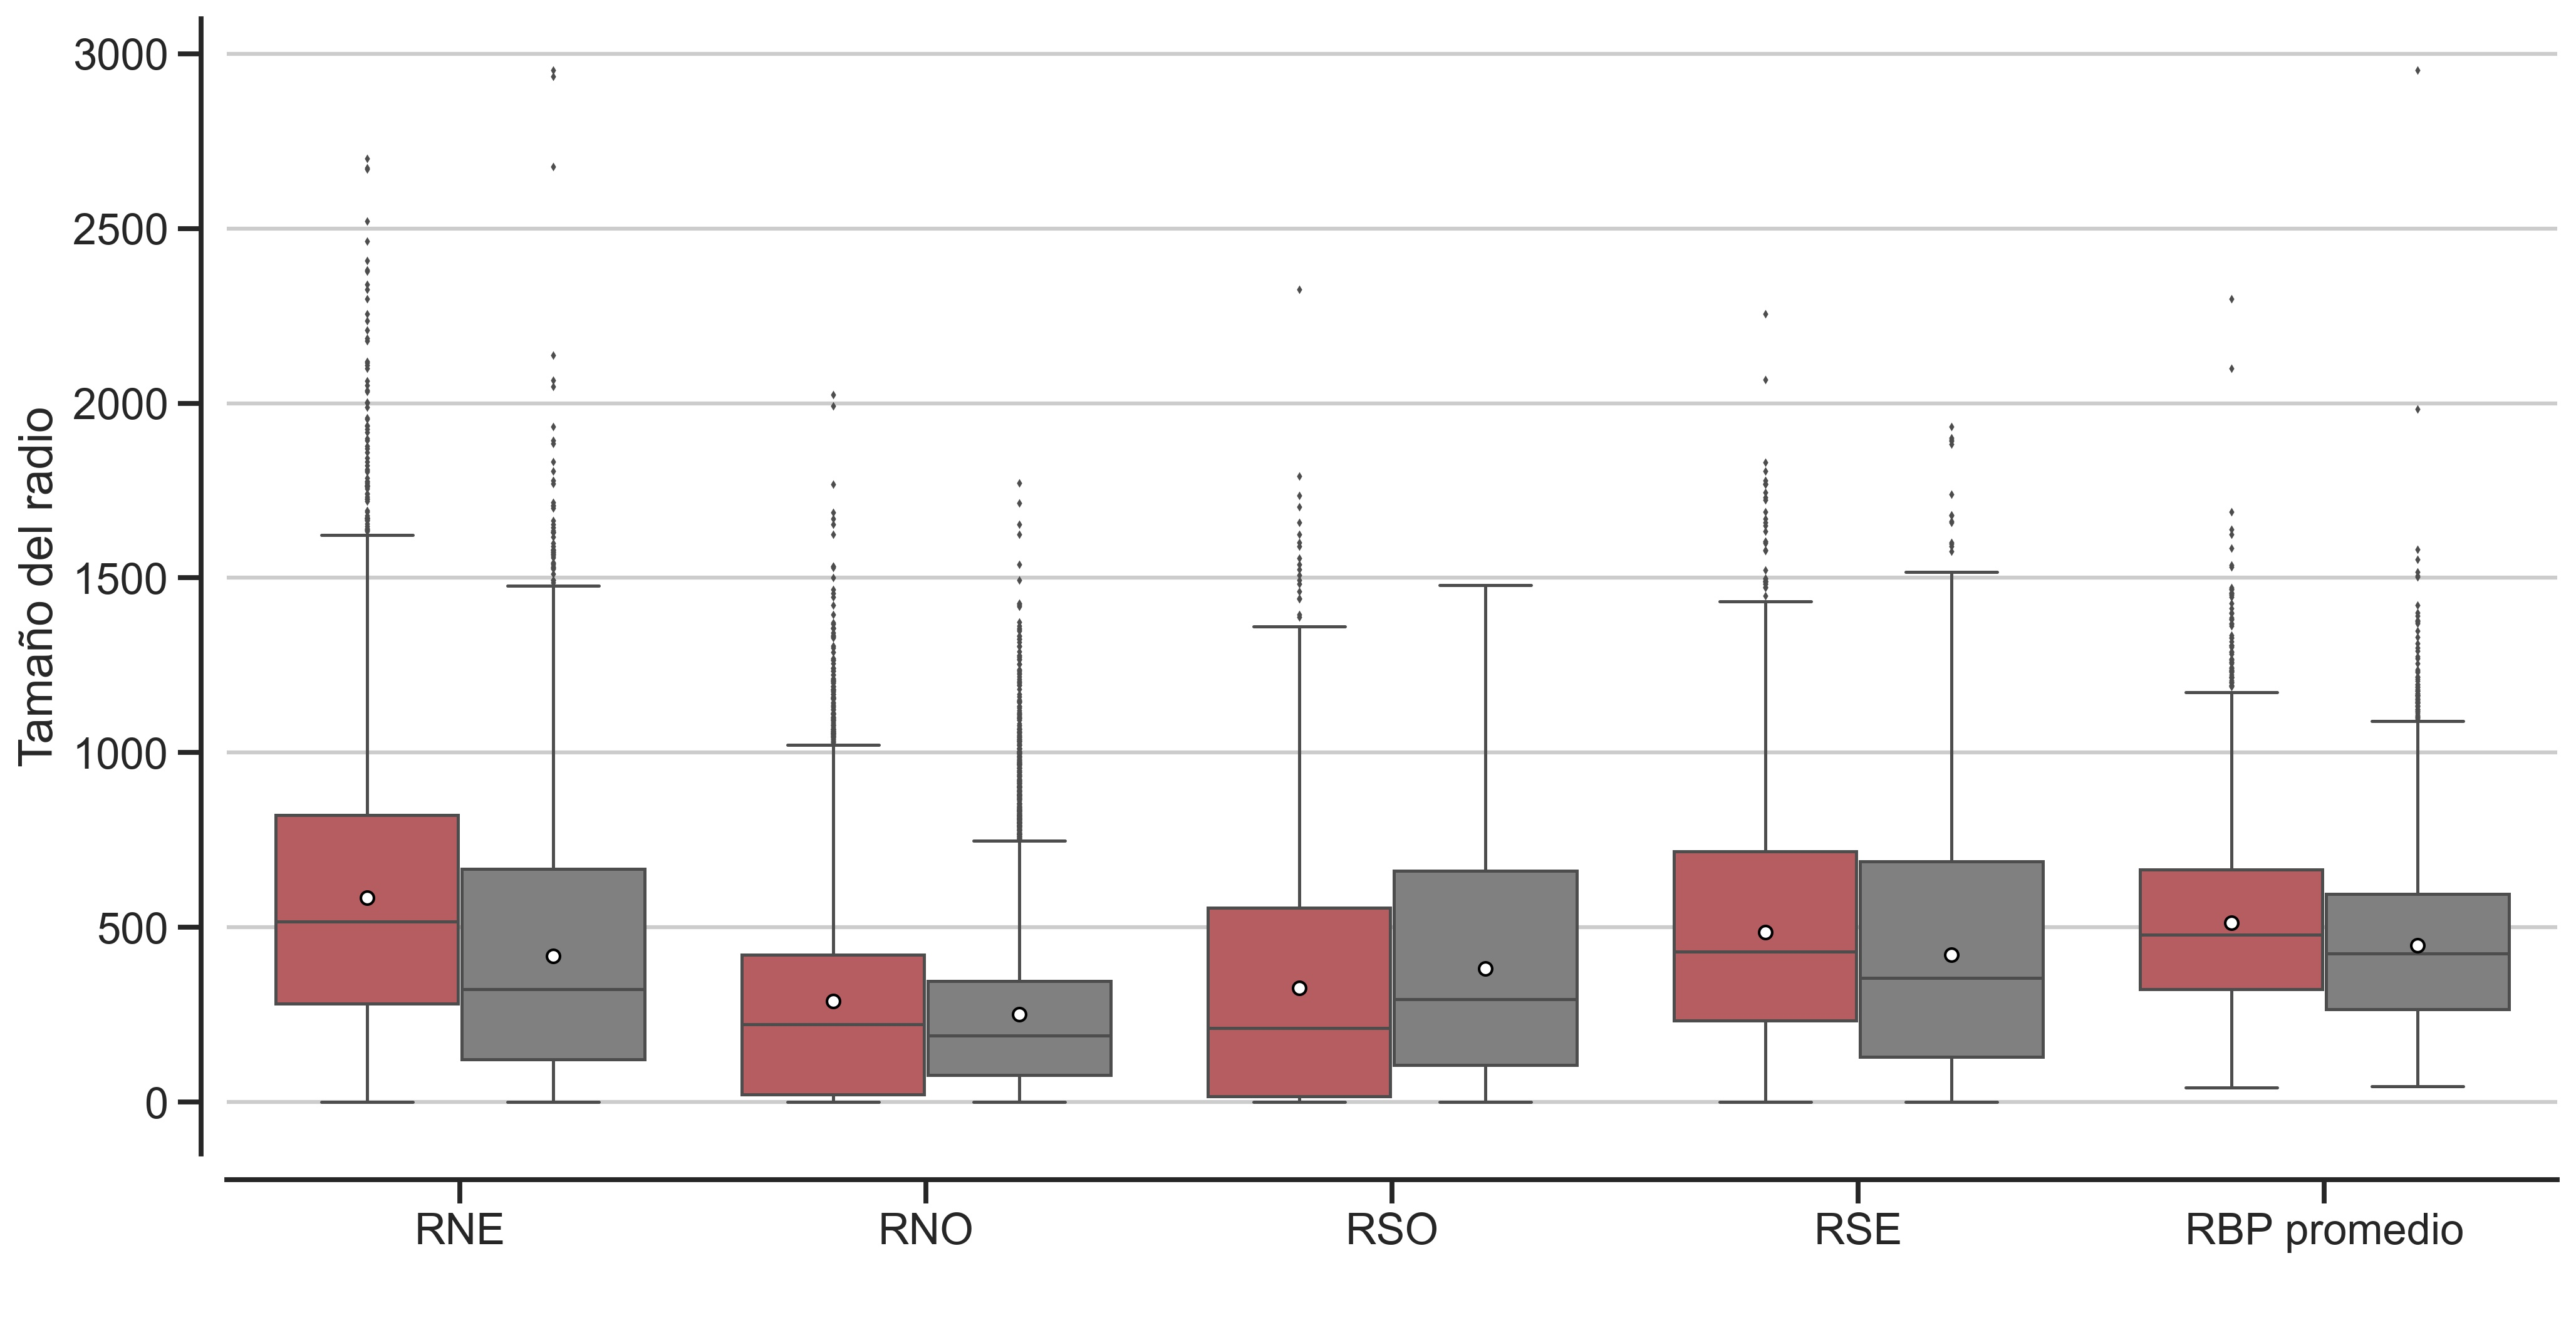
\includegraphics[scale = 0.3]{Images/Figures/Fig_3_13.jpeg}
        \caption{Cajas y bigotes de las distribuciones de los radios por cuadrante y el $R_p$ (km) de los radios en la región de estudio de la cuenca {\red NA} y {\gray EP} definidos por el algoritmo RBP.}
        \label{fig:fig_13}
    \end{figure}
\end{frame}

\begin{frame}
    \begin{exampleblock}{Correlaciones para el NA}
        % Please add the following required packages to your document preamble:
% \usepackage{booktabs}
% \usepackage{graphicx}
\begin{table}[H]
\centering
\caption{Correlación de rango de Spearman (r) entre los tamaños calculados con las técnicas de ROCLOUD y RBP para cada cuadrante y promedio; Se determinan para la cuenca NA. Los valores con un asterisco son significativos a un nivel del 95\% de confianza.}
\label{tab:3.5}
\resizebox{\textwidth}{!}{%
\begin{tabular}{@{}llllll@{}}
\toprule
             & RNE\_RPB       & RNO\_RPB       & RSO\_RPB       & RSE\_RPB       & Rp\_RPB        \\ \midrule
RNE\_ROCLOUD & \textit{0.81*} &                &                &                &                \\
RNO\_ROCLOUD & \textit{0.14}  & \textit{0.67*} &                &                &                \\
RSO\_ROCLOUD & \textit{0.05}  & \textit{0.17}  & \textit{0.63*} &                &                \\
RSE\_ROCLOUD & \textit{0.32*} & \textit{0.09}  & \textit{0.18}  & \textit{0.66*} &                \\
Rp\_ROCLOUD  & \textit{0.59*} & \textit{0.32*} & \textit{0.37*} & \textit{0.5*}  & \textit{0.73*} \\ \bottomrule
\end{tabular}%
}
\end{table}
    \end{exampleblock}
\end{frame}

\begin{frame}
    \begin{alertblock}{Correlaciones para el EP}
        % Please add the following required packages to your document preamble:
% \usepackage{booktabs}
% \usepackage{graphicx}
\begin{table}[H]
\centering
\caption{Igual a la Cuadro \ref{tab:3.5}, pero para el EP}
\label{tab:3.6}
\resizebox{\textwidth}{!}{%
\begin{tabular}{@{}llllll@{}}
\toprule
             & RNE\_RPB       & RNO\_RPB       & RSO\_RPB       & RSE\_RPB       & Rp\_RPB        \\ \midrule
RNE\_ROCLOUD & \textit{0.77*} &                &                &                &                \\
RNO\_ROCLOUD & \textit{0.32*} & \textit{0.71*} &                &                &                \\
RSO\_ROCLOUD & \textit{0.12}  & \textit{0.21}  & \textit{0.69*} &                &                \\
RSE\_ROCLOUD & \textit{0.26}  & \textit{0.08}  & \textit{0.28}  & \textit{0.67*} &                \\
Rp\_ROCLOUD  & \textit{0.56*} & \textit{0.38*} & \textit{0.48*} & \textit{0.57*} & \textit{0.74*} \\ \bottomrule
\end{tabular}%
}
\end{table}
    \end{alertblock}
\end{frame}

\begin{frame}
\begin{enumerate}
\setcounter{enumi}{1}
    \item Dependencia de la PCT con el tamaño del CT: GPM\_MERGIR
\end{enumerate}
    \begin{columns}
        \begin{column}{0.6\textwidth}
        \begin{figure}
            \centering
            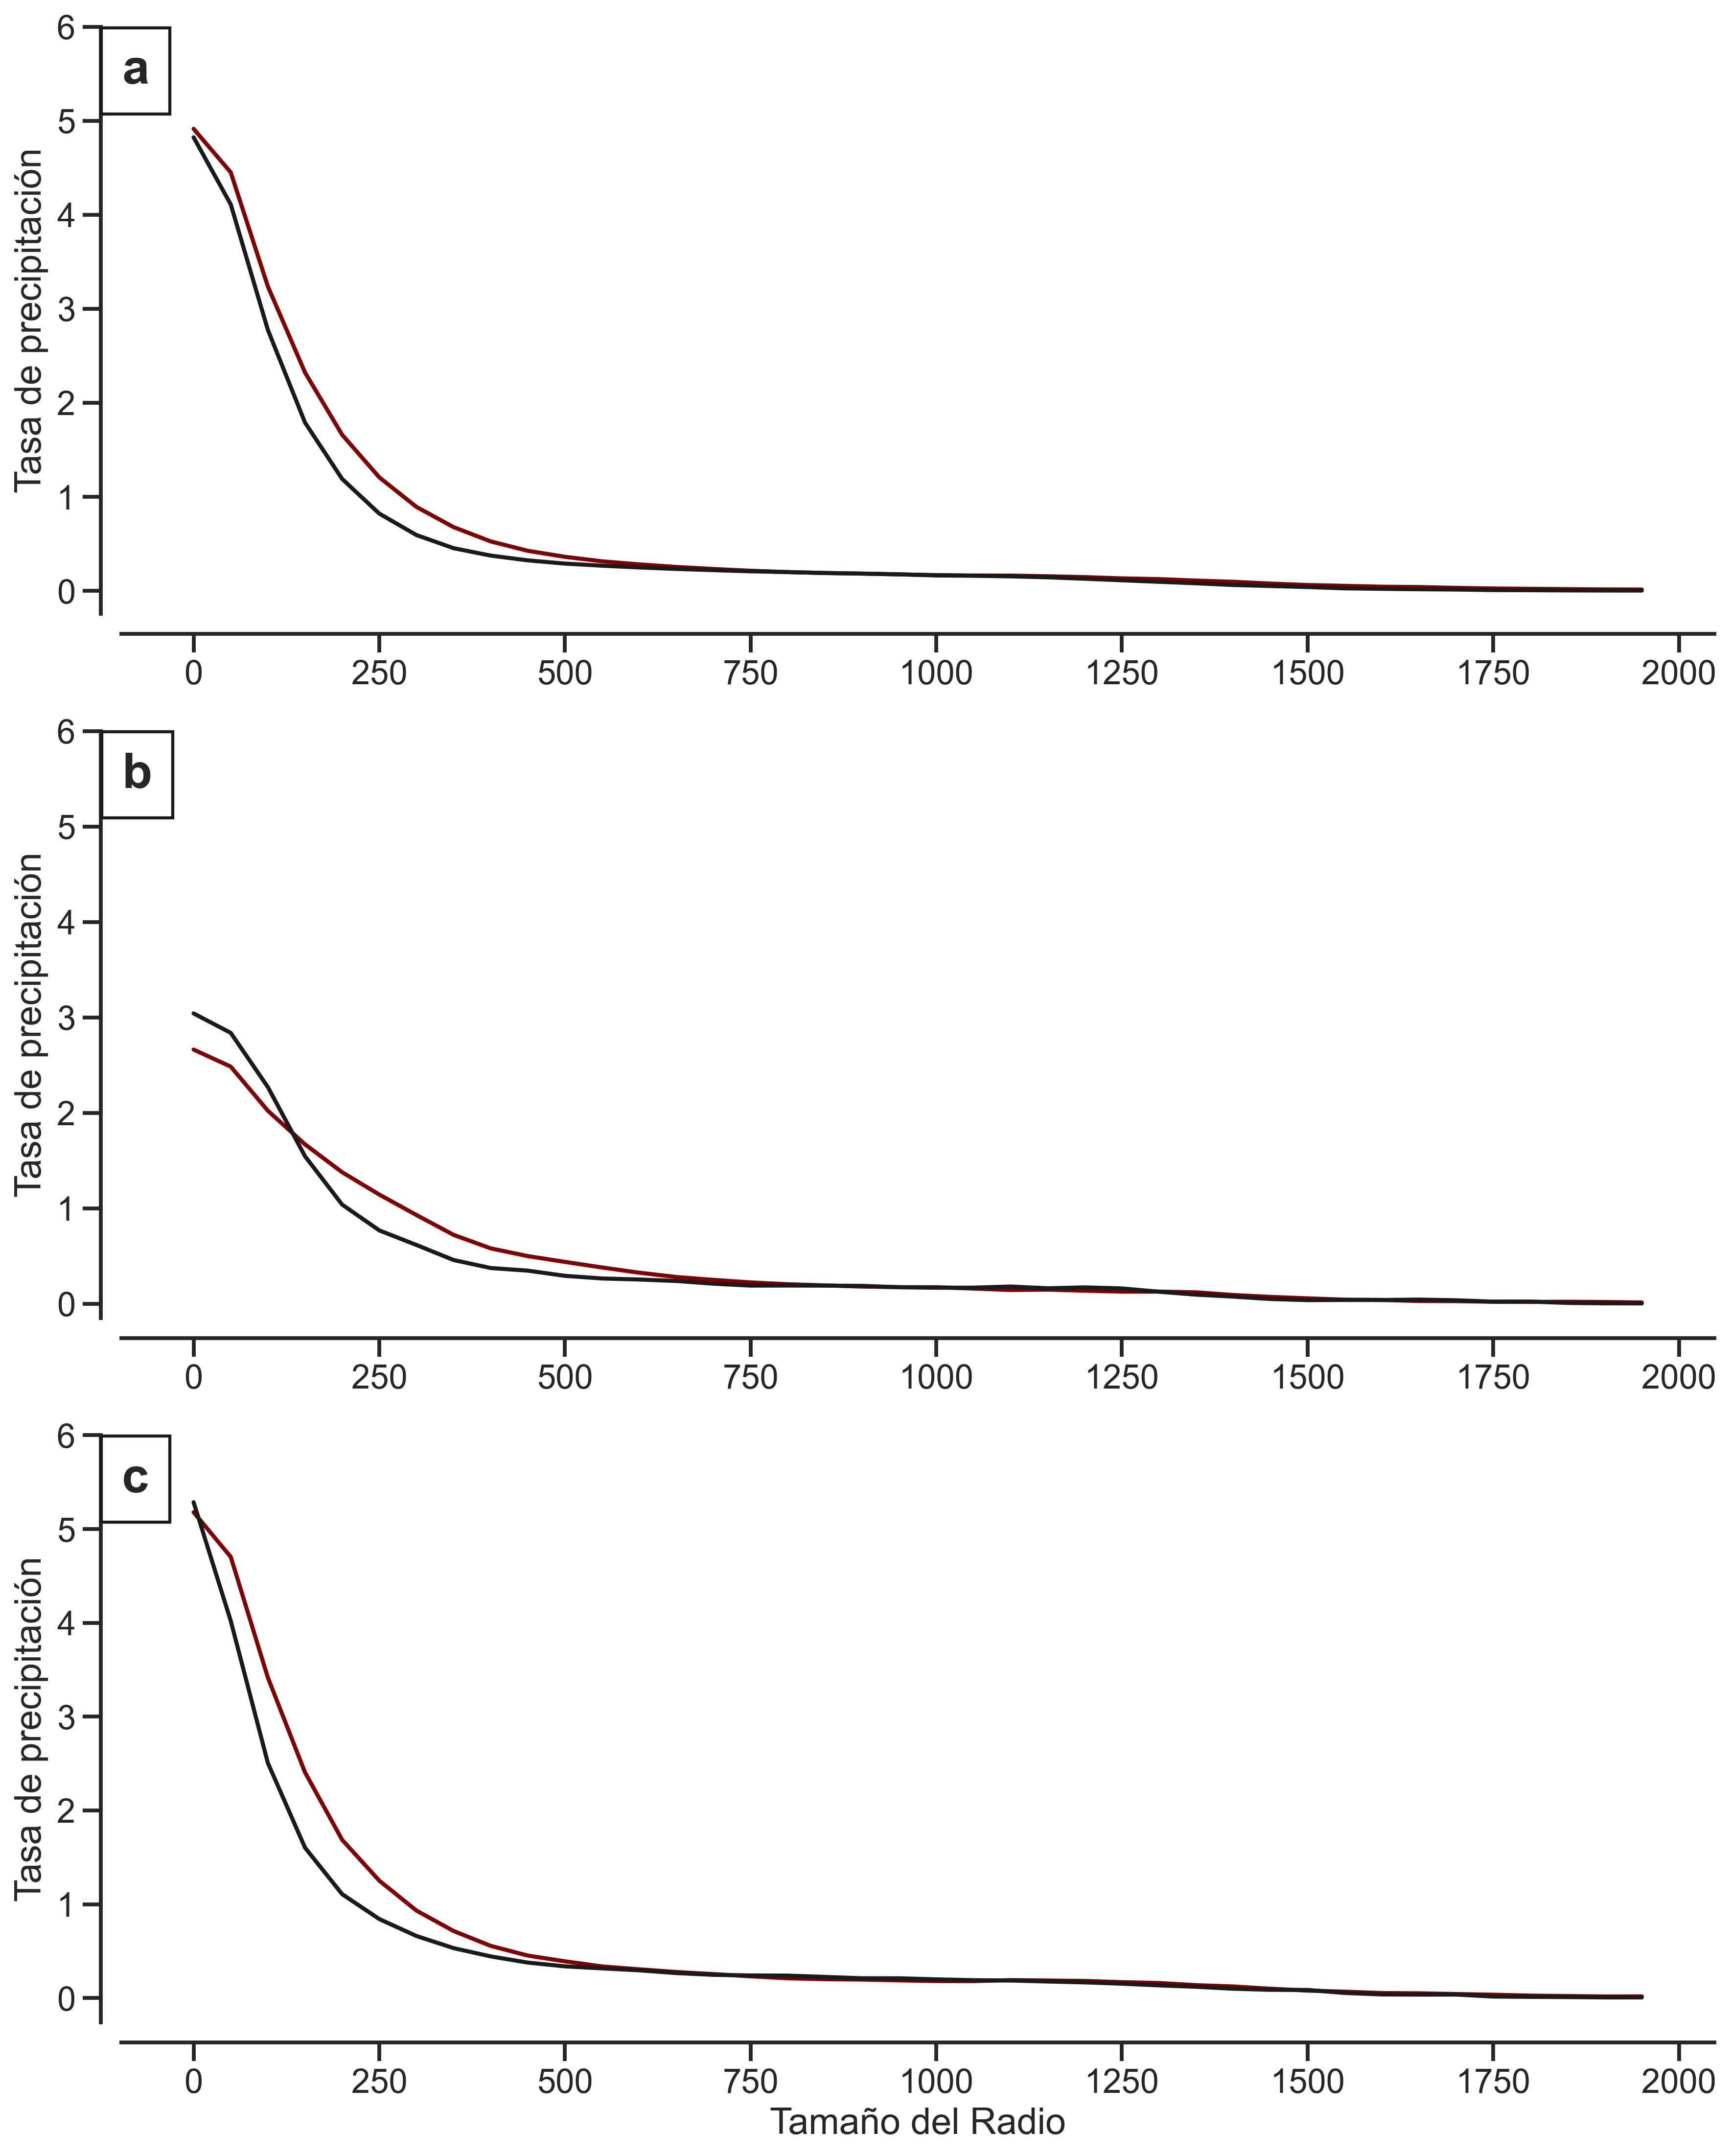
\includegraphics[scale = 0.22]{Images/Figures/Fig_3_16.jpeg}
            \caption{}
            \label{fig:fig_rbp}
        \end{figure}
        \end{column}
        
        \begin{column}{0.4\textwidth}
            \begin{block}{Figura 13:}
                Tasa de precipitación ($mm h^{-1}$) de IMERG del CT en función del radio (km), medido por la técnica de anillos, para (a) todas las posiciones, (b) posiciones sobre continente y (c) posiciones que se encuentren al menos a 250 km de la costa.
            \end{block}
        \end{column}
    \end{columns}
\end{frame}

\begin{frame}
\begin{enumerate}
\setcounter{enumi}{2}
    \item Dependencia de la PCT con el tamaño del CT: CHIRPS
\end{enumerate}
    \begin{figure}
        \centering
        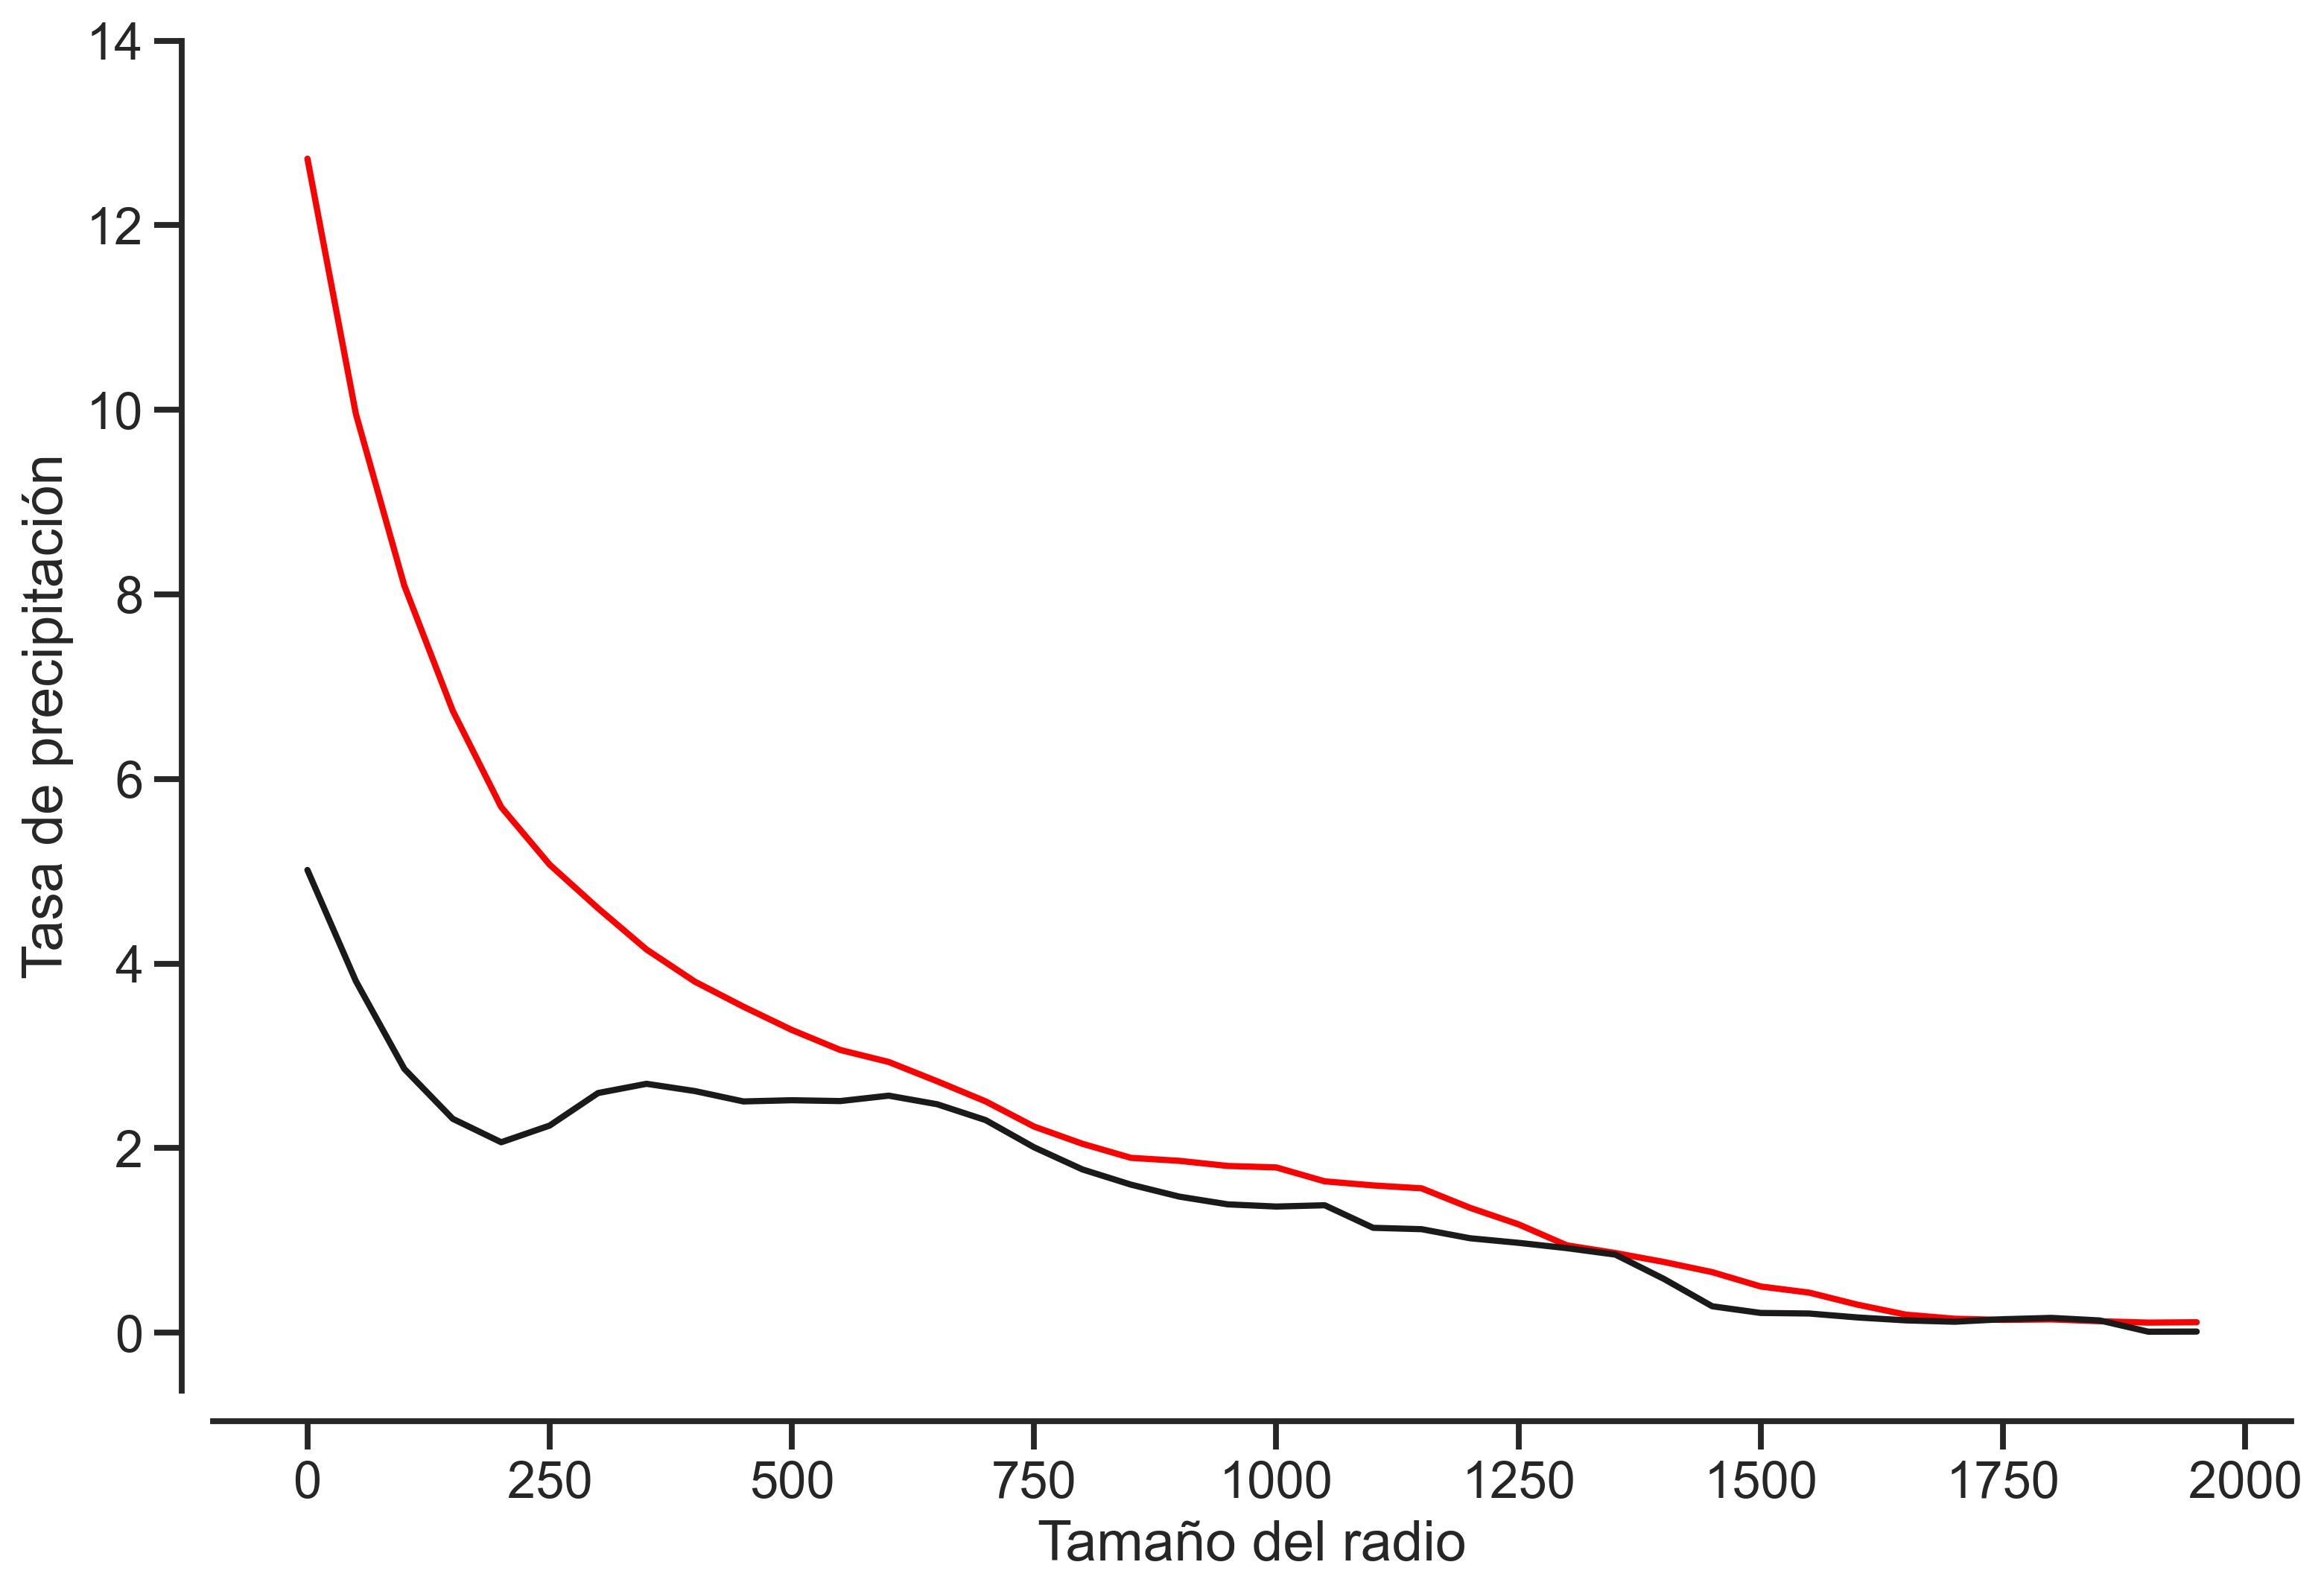
\includegraphics[scale = 0.35]{Images/Figures/Fig_3_21.jpeg}
        \caption{Tasa de precipitación (mm $h^{-1}$) del CTs en función de su tamaño (km), definido por los rangos intercuartílicos del tamaño definido por ROCLOUD, en las cuencas: (a) {\red NA} y (b) {\gray EP}.}
        \label{fig:figchirps}
    \end{figure}
\end{frame}

\subsection{Sobre las variables medioambientales y la precipitación}
\begin{frame}
\begin{itemize}
    \item Algunos CT muestran una fuerte divergencia en la atmósfera superior. Puede estar relacionado con grandes cantidades de humedad en la atmósfera de nivel medio, lo que produce tasas de precipitación intensas de CT en la superficie.

    \item Los CTs en ambientes secos producen menos precipitación y tienen menores extensiones radiales de viento en comparación con los CTs en ambientes húmedos.

    \item La cizalladura del viento es más importante para los CT sobre la cuenca de {\red NA}. Esto último está posiblemente relacionado con el hecho de que las trayectorias de los CT cerca de la masa continental son modificadas por la cizalladura ambiental.

    \item Ni la intensidad del CT ni la presión central a nivel del mar son importantes para la estimación de la precipitación del CT, situado dentro del tamaño exterior del CT.
\end{itemize}
\end{frame}

\subsection{Sobre la forma del CT}
\begin{frame}
\begin{figure}
    \centering
    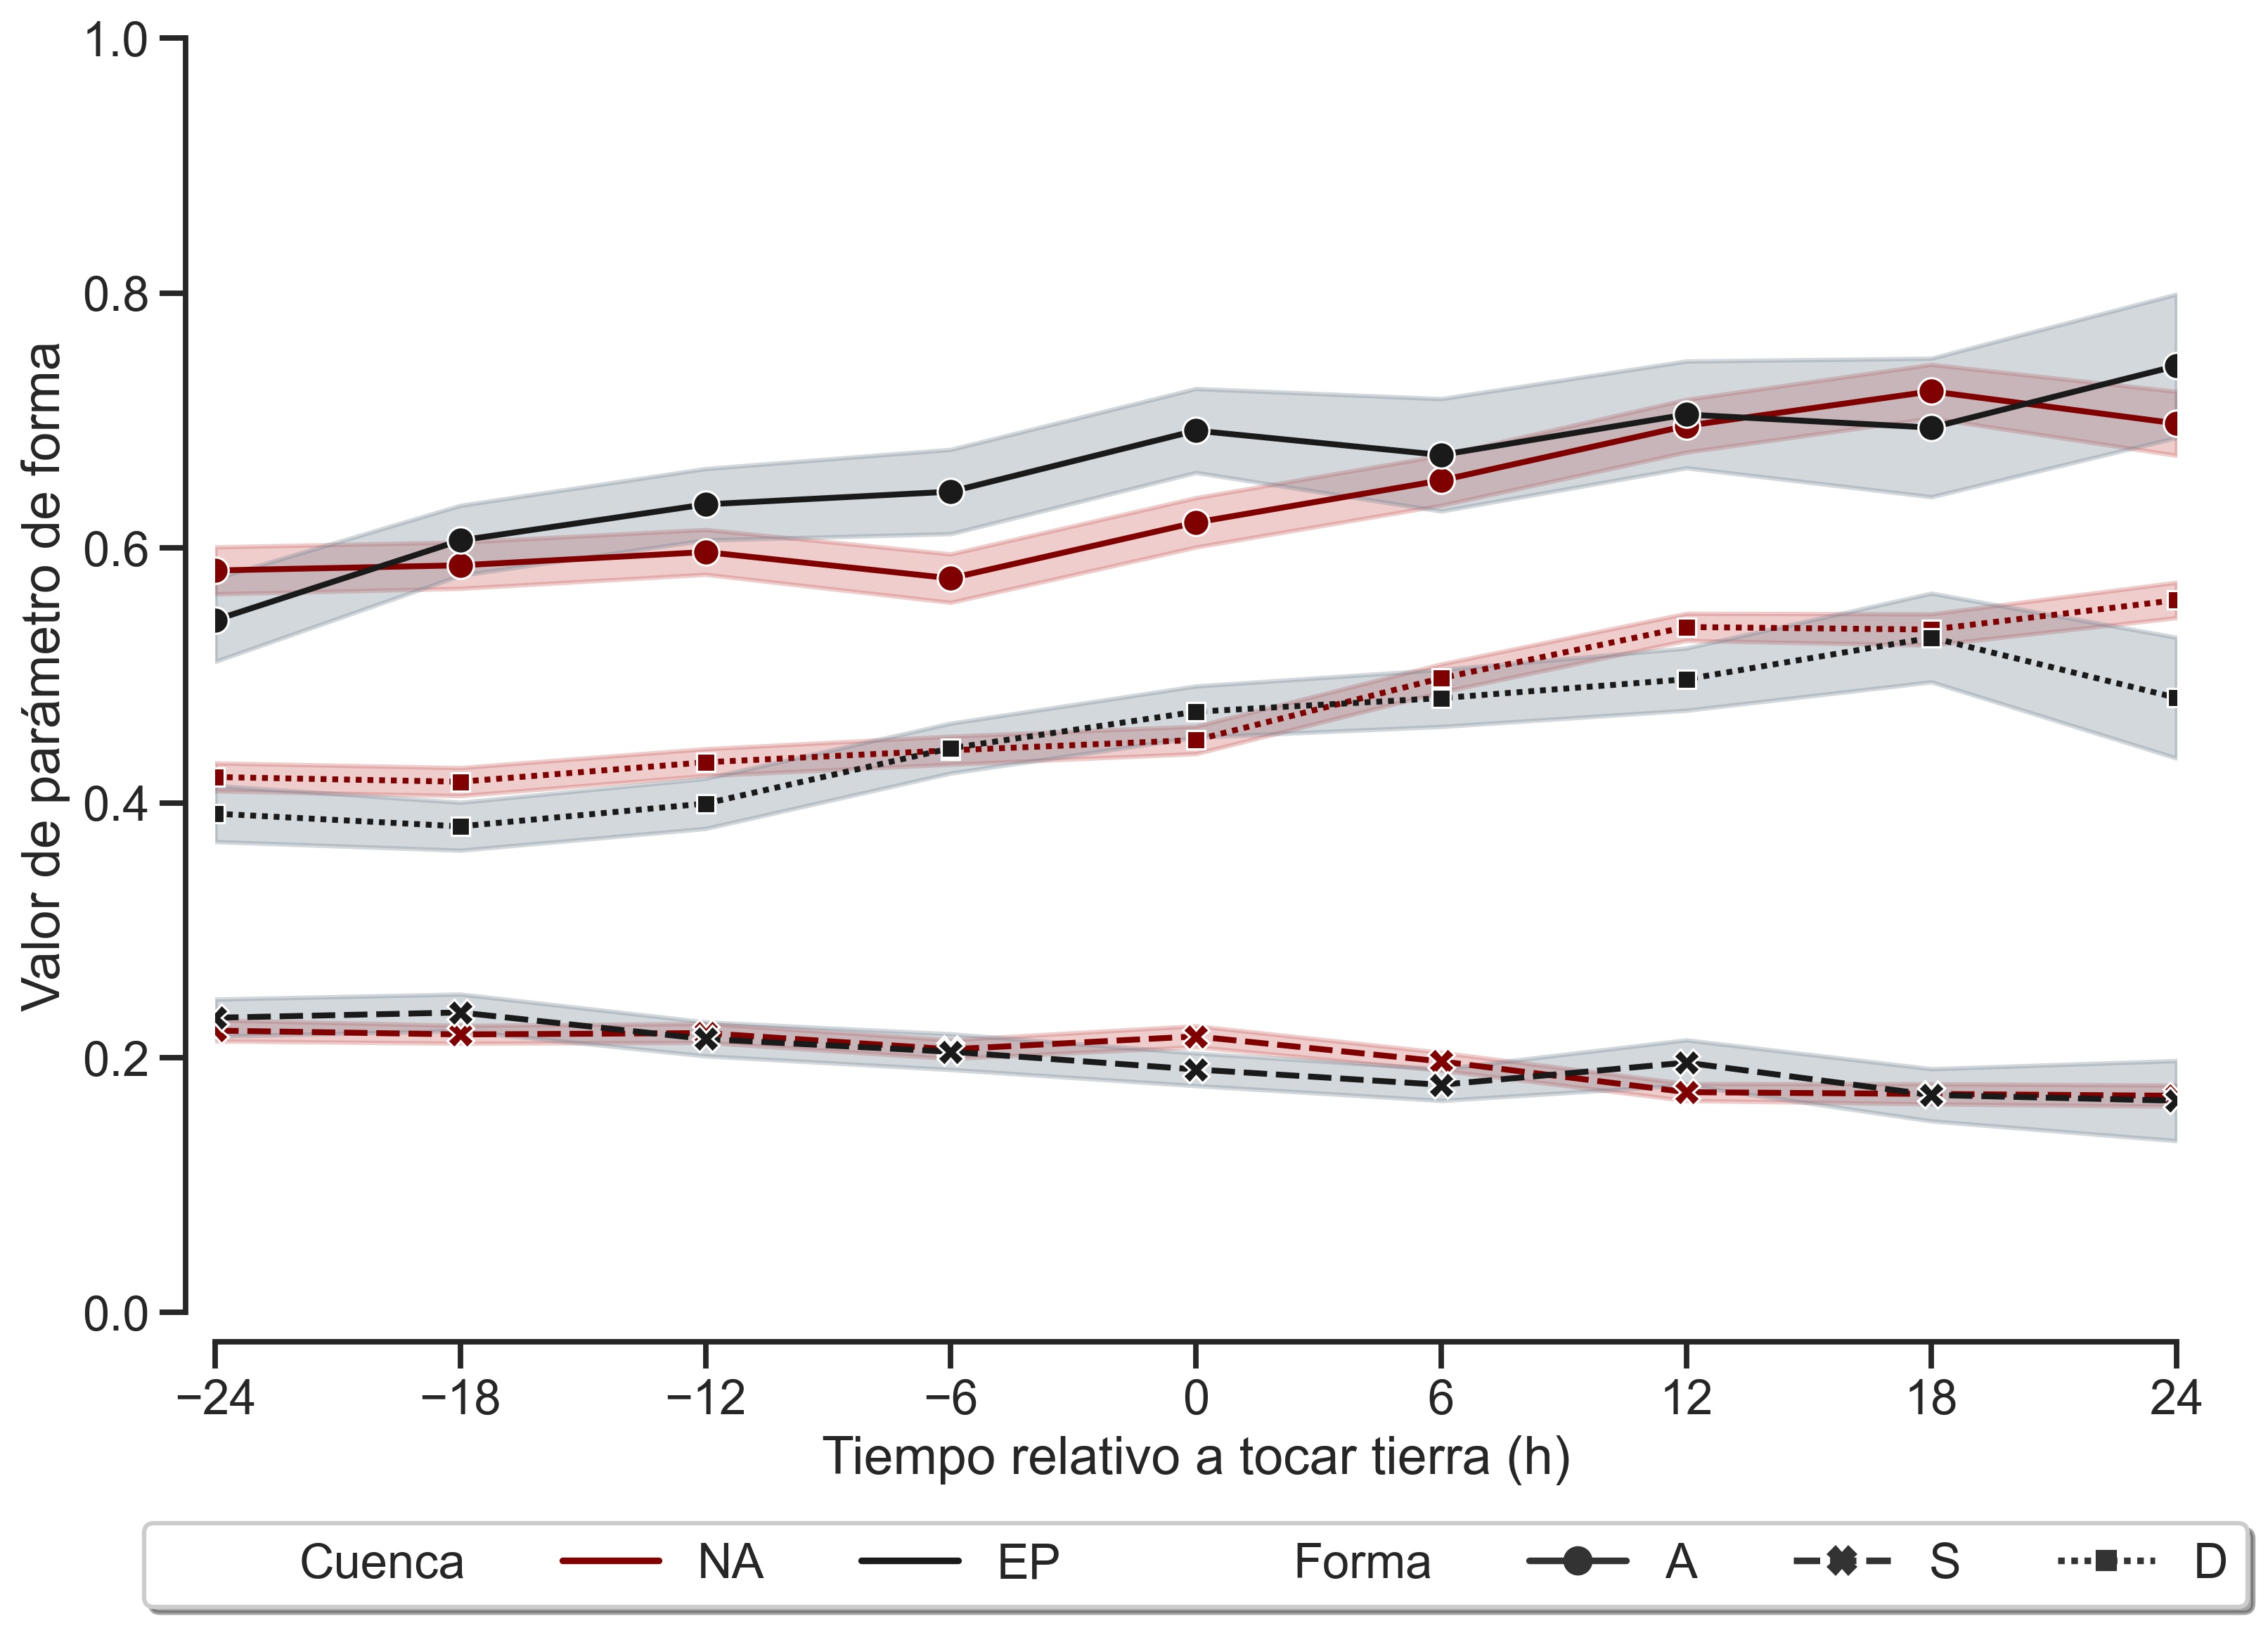
\includegraphics[scale = 0.3]{Images/Figures/Fig_3_32.jpeg}
    \caption{Comportamiento promedio de las métricas de forma de los CTs de la cuenca {\red NA} y {\gray EP}, 24h antes (-24) y 24h después (24) de hacer \textit{landfalling}.}
    \label{fig:fig_10}
\end{figure}
\end{frame}